\chapter{SS19}\label{ch:klausurss19}

\section{Aufgabe 1}

Bei der Aufgabe ist es wichtig, die Anforderungen genau zu beachten.\\
Ob eine Thread die while-wait-Schleife verlassen darf, wird von der Methode \code{tick()} gesteuert - wieviele Ticks ein Thread in der Schleife bleiben soll, wird von dem jeweiligen Thread definiert.\\
Die \code{tick()}-Methode wird von anderen Threads aufgerufen, es kann also durchaus vorkommen, dass mehrmals hintereinander
die \code{notifyAll()}-Methode aufgerufen wird - diese entfernt alle Threads aus der Warteschlange, damit die Threads ihre
Wartebedingungen erneut überprüfen können.\\
da \code{tick()} aber auch gleichzeitig einen Zähler realisieren soll, \textit{muss} es in der Methode auch eine Zählvariable geben, anhand derer die in der while-wait-Schleife enthaltenen Threads feststellen können, wie oft \code{tick()} aufgerufen wurde, um entsprechend aus der Schleife und nachfolgend der Methode herauszukommen.

\begin{figure}
    \centering
    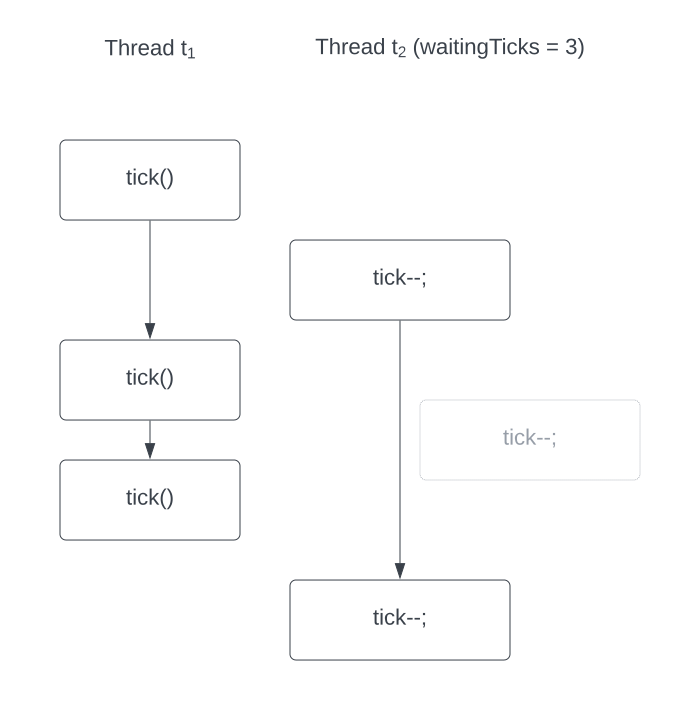
\includegraphics[scale=0.5]{chapters/Anhang/Klausuren/img/tick}
    \caption{Thread $t_1$ ruft 3 mal \texit{tick()} auf. Den Anforderungen nach müsste Thread $t_2$ danach aus der while-wait-Schleife herauskommen, erhält aber nicht die Sperre auf das Objekt von LogicalTime, um seinen eigenen Zähler rechtzeitig zu erniedrigen, bevor $t_1$ erneut \textit{tick()} aufruft. (Quelle: eigene)}
    \label{fig:tick}
\end{figure}

\section{Aufgabe 6}
Auch hier gilt, dass die Aufgabenstellung aufmerksam zu lesen ist.\\
Der Kreis soll erst ausgefüllt werden, wenn die Maustaste gelöst wird.

\begin{minted}[mathescape,
    linenos,
    numbersep=5pt,
    gobble=2,
    frame=lines,
    framesep=2mm]{java}
    private void mousePressed(double x, double y) {
        c = new Circle();
        c.setCenterX(x);
        c.setCenterY(y);
        c.setStroke(Color.RED);
        c.setFill(null); // oder Color.TRANSPARENT
        c.setRadius(RADIUS);
        graphicsPane.getChildren().add(c);
    }

    private void mouseReleased() {
        c.setFill(Color.RED);
        c = null;
    }
\end{minted}

\section{Aufgabe 8}

In der Abbildung \ref{fig:batchmodus} ist links der sequentielle Modus dargestellt, bei dem nach dem Senden einer Nachricht auf die Antwort des Servers gewartet wird, bevor eine neue Nachricht geschickt wird.
Dies wird i.d.R. verwendet, wenn das Senden einer neuen Nachricht abhängig ist von einem Ergebnis, die über die Server-Antwort übermittelt wird, oder wenn mit dem Server interagiert wird (Request abhängig vom Response).\\
Der Batch-Modus auf der rechten Seite der gleichen Abbildung ist schneller, da zwischen dem Senden von Nachrichten nicht auf Antworten gewartet werden müssen. \\
Erst nach dem Senden eine Batches von Nachrichten werden die dem Client zur Verfügung stehenden Antworten ausgelesen.\\

\noindent
In dieser Form des Batch-Modus besteht allerdings die Gefahr, dass es zu Verklemmungen kommt:
\begin{itemize}
    \item Bei dem Client kommen viele Nachrichten an, während er noch sendet.
    \item Die ankommenden Nachrichten für den Client werden gepuffert, bis sie ausgelesen werden (TCP- / OS-seitig).
    \item Läuft der Puffer voll, sorgt die Flusskontrolle (TCP) dafür, dass dem Sender mitgeteilt wird, dass keine Nachrichten mehr empfangen werden können, der Server sendet nicht mehr.
    \item Die zu sendenden Nachrichten des Servers werden in einen Puffer geschrieben.
    \item Der Sende-Puffer des Senders läuft voll.
    \item Bei dem nächsten Sende-Aufruf blockiert der Server, empfangene Nachrichten landen im Empfangspuffer
    \item Der Empfangspuffer des Servers läuft voll, der Client buffert die zu sendenden Nachrichten.
    \item Beide Anwendungen blockieren.
\end{itemize}

\\noindent
Um dieses Problem beim Batch-Modus zu umgehen, werden für das Senden und Empfangen zwei Threads auf Client-Seite erstellt: Ein Thread sendet, ein Thread empfängt. \\
Dadurch kann von dem Client immer wieder sein Empfangspuffer geleert werden, der Server wird beim Senden nicht blockiert.

\begin{figure}
    \centering
    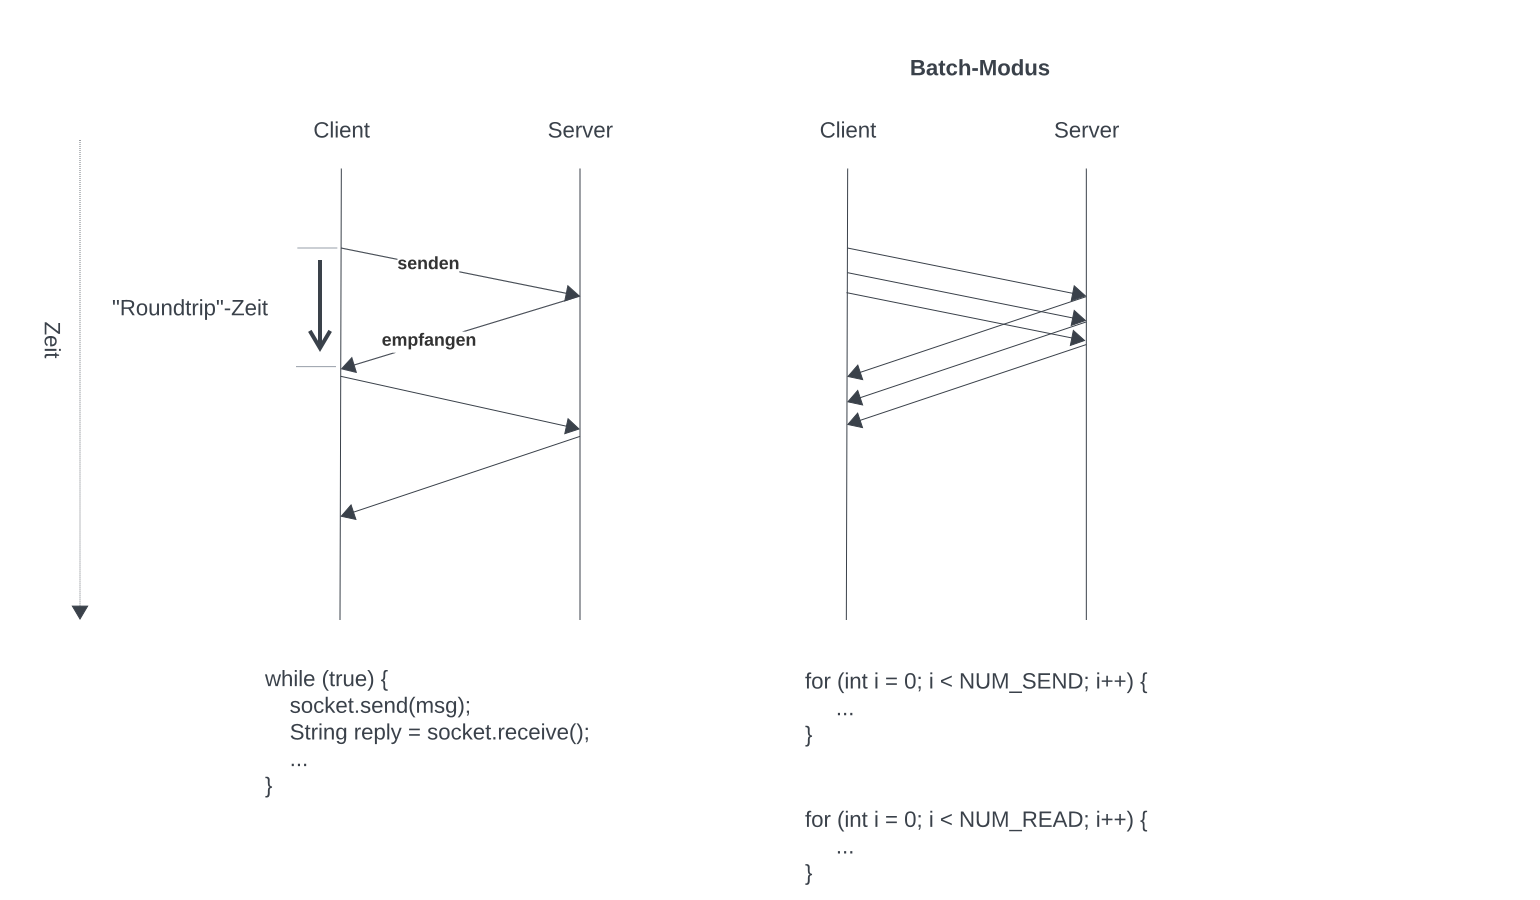
\includegraphics[scale=0.4]{chapters/Anhang/Klausuren/img/batchmodus}
    \caption{Vereinfachte Darstellung sequentieller Kommunikation und Batch-Modus (Quelle: eigene)}
    \label{fig:batchmodus}
\end{figure}